\documentclass[runningheads]{llncs}

\usepackage[T1]{fontenc}
\usepackage{lmodern}
\usepackage{booktabs}
\usepackage{microtype}
\usepackage{graphicx}
\usepackage{amsmath}
\usepackage{siunitx}
\usepackage{xcolor}
\usepackage{tikz}
\usepackage{pgfplots}
\usepackage{xurl}
\usepackage[hidelinks]{hyperref}
\setlength{\emergencystretch}{1em}
\usetikzlibrary{arrows.meta,positioning,matrix}
\pgfplotsset{compat=1.18}

\definecolor{ChronoInk}{HTML}{1F2937}
\definecolor{ChronoMuted}{HTML}{5B6573}
\definecolor{ChronoBlue}{HTML}{1769AA}
\definecolor{ChronoBlueLight}{HTML}{9CC9E8}
\definecolor{ChronoOrange}{HTML}{C65D00}
\definecolor{ChronoPale}{HTML}{E8F2F8}
\definecolor{ChronoGrid}{HTML}{AEB8C2}
\AtBeginDocument{\color{ChronoInk}}
\hypersetup{colorlinks=true,linkcolor=ChronoBlue,citecolor=ChronoBlue,urlcolor=ChronoBlue}

\newcommand{\ScreenedFamilyCount}{67}
\newcommand{\SupportedFamilyCount}{54}
\newcommand{\ReviewFamilyCount}{7}
\newcommand{\FailedFamilyCount}{6}
\newcommand{\TrainingFamilyCount}{22}
\newcommand{\OriginalDevelopmentFamilyCount}{12}
\newcommand{\TestFamilyCount}{16}
\newcommand{\ReserveFamilyCount}{4}
\newcommand{\OptimizerRunCount}{5}
\newcommand{\OptimizerCandidateCount}{32}
\newcommand{\OptimizerGameCount}{4,680}
\newcommand{\ChampionshipGameCount}{2,112}
\newcommand{\DevelopmentGameCount}{440}
\newcommand{\ConfirmatoryGameCount}{512}
\newcommand{\MechanismGameCount}{480}
\newcommand{\ComponentGameCount}{480}
\newcommand{\TotalGameCount}{8,704}
\newcommand{\AcceptedAllocationCount}{562}
\newcommand{\AcceptedCoreHours}{288.72}
\newcommand{\AcceptedRequestedMemoryGiB}{6}
\newcommand{\AcceptedPeakRSSGiB}{1.63}
\newcommand{\DefaultScore}{0.199}
\newcommand{\ChampionScore}{0.535}
\newcommand{\ImprovementEstimate}{0.336}
\newcommand{\ImprovementSE}{0.057}
\newcommand{\ImprovementCILower}{0.215}
\newcommand{\ImprovementCIUpper}{0.457}
\newcommand{\ChampionAbsoluteMargin}{0.035}
\newcommand{\ChampionAbsoluteLower}{-0.021}
\newcommand{\DefaultWins}{1}
\newcommand{\DefaultDraws}{100}
\newcommand{\DefaultLosses}{155}
\newcommand{\ChampionWins}{47}
\newcommand{\ChampionDraws}{180}
\newcommand{\ChampionLosses}{29}
\newcommand{\PositiveFamilyCount}{14}
\newcommand{\ZeroFamilyCount}{2}
\newcommand{\NegativeFamilyCount}{0}
\newcommand{\ImprovementBootstrapLower}{0.230}
\newcommand{\ImprovementBootstrapUpper}{0.447}
\newcommand{\ImprovementSignFlipP}{0.000122}
\newcommand{\MechanismEstimate}{0.083}
\newcommand{\MechanismCILower}{-0.027}
\newcommand{\MechanismCIUpper}{0.192}
\newcommand{\ComponentAverageEstimate}{0.057}
\newcommand{\ComponentAverageCILower}{-0.003}
\newcommand{\ComponentAverageCIUpper}{0.118}
\newcommand{\StrategyEstimate}{0.331}
\newcommand{\StrategyOrdinaryLower}{0.096}
\newcommand{\StrategyOrdinaryUpper}{0.567}
\newcommand{\StrategyFamilywiseLower}{-0.007}
\newcommand{\StrategyFamilywiseUpper}{0.670}
\newcommand{\ImprovedPairCount}{150}
\newcommand{\RegressedPairCount}{6}
\newcommand{\UnchangedPairCount}{100}
\newcommand{\StableDrawPairCount}{76}
\newcommand{\StableDrawCombatantDifference}{22.71}
\newcommand{\StableDrawUnitDifference}{12.43}
\newcommand{\StableDrawCreditDifference}{-683.82}


\title{Leakage-Resistant Evaluation of Scripted RTS Agent Configuration in
Chrono Divide}
\titlerunning{Leakage-Resistant Scripted RTS Agent Evaluation}
\author{Anonymous Author(s)}
\authorrunning{Anonymous Author(s)}
\institute{Anonymous institution}

\begin{document}
\maketitle

\begin{abstract}
Scripted game-agent gains can reflect map memorization, favorable starts,
uncontrolled randomness, or contaminated baselines. We present a
leakage-resistant evaluation protocol and reproducible configuration pipeline
for StrongBot in Chrono Divide, an existing browser reconstruction of
\emph{Command \& Conquer: Red Alert 2}.
Revision-aware map families, outcome-free compatibility screens, an isolated
pinned opponent, participant-specific random streams, reciprocal starts,
sealed tests, and provenance commitments form a joint evidence contract: a
campaign is admitted only if every commitment matches its frozen
plan. Five \OptimizerCandidateCount{}-policy deterministic searches with
successive halving use training families; a common-seed championship selects one
coordinate-free policy. In \ConfirmatoryGameCount{} games over
\TestFamilyCount{} sealed families, the champion scores \ChampionScore{} versus
\DefaultScore{} for a frozen generic reference. The
equal-family improvement is \ImprovementEstimate{}
(family-clustered 95\% CI
[\ImprovementCILower{},~\ImprovementCIUpper{}]);
\PositiveFamilyCount{} family effects are positive and \ZeroFamilyCount{} are
zero. The prespecified joint objective fails: the absolute-strength
gate's one-sided 95\%
lower bound for the champion's margin above 0.5 is
\ChampionAbsoluteLower{}. Improvement primarily replaces losses with survival
or wins. The study establishes improvement within this policy class, not
superiority over Supalosa, the deployed default, other opponents or matchups.
The contract makes the result bounded and auditable. An identity-neutral
artifact regenerates every table and figure.

\keywords{game artificial intelligence \and real-time strategy games \and
scripted agents \and agent evaluation \and reproducible simulation}
\end{abstract}

\section{Introduction}
\label{sec:introduction}

Full-game real-time strategy (RTS) agents must coordinate economy, production,
scouting, defense, force composition, movement, and terminal objective
completion over thousands of updates. The same complexity makes evaluation
fragile. A bot may appear stronger because it was tuned on the reported map,
received a favorable physical start, consumed a lucky or coupled random stream,
or faced an opponent loaded from the candidate's modified dependency tree.
Short-game resignation is another hidden variable: it can award a nominal win
before the literal game objective is achieved.

We study these problems in Chrono Divide, an existing ground-up browser
reconstruction of \emph{Command \& Conquer: Red Alert 2} with a programmable
offline bot API~\cite{chronodivide2026,chronodivideGameApi2026}. Chrono Divide
is not introduced by this paper. We use it as a practical full-game simulation
environment and develop StrongBot from Supalosa's public scripted
agent~\cite{supalosa2026bot}. The research question is deliberately concrete:
can an auditable development process produce a bot that reliably beats the
pinned external Supalosa implementation under literal all-building elimination,
without reducing the claim to one country, start, slot, or favorable replay?

Exploration revealed that one global policy was not enough. Heck Freezes Over
(HFO) has four asymmetric physical starts. The west start required early
rush-oriented production plus a grouped home guard; the bottom start produced
long draws in which attack groups repeatedly failed to finish a small remaining
base. StrongBot therefore uses narrowly scoped policy layers: country-aware west
rush/guard profiles, a progress-gated bottom building-retarget controller, and
late literal closeout logic. Each layer was selected on fresh cases, replicated,
and then required to be action- and state-identical outside its declared map,
start, and faction boundary. Only after those gates passed was the complete
deployed bot frozen for all-country, all-start confirmation.

A second map exposed a different failure. On Peak of Perfection the same macro
profile was applied at one physical start but not its reciprocal. A frozen
$2\times2$ scope study separated macro-strategy scope from tactical-scope
changes. The selected change applies the existing macro profile at both starts
while leaving the tactical layer unchanged. Fresh replication then tests
whether this simple spatial repair generalizes across all countries and slots.

We organize the empirical questions as follows:

\begin{enumerate}
  \item[RQ1.] Does frozen StrongBot reliably beat pinned Supalosa on HFO under
  balanced countries, four physical starts, both participant slots, and the
  literal objective?
  \item[RQ2.] Which scoped mechanisms account for the difficult HFO conditions,
  and are they exactly inactive outside their declared conditions?
  \item[RQ3.] Does reciprocal macro-profile scope repair Peak of Perfection on
  fresh balanced cases?
  \item[RQ4.] Does HFO strength transfer to an independently sourced RA2Web
  Advanced opponent?
\end{enumerate}

The answer is strong but bounded. StrongBot wins 633 of 720 HFO games, with
pooled and country-by-start lower bounds above 0.84. The Peak reciprocal policy
wins 134 of 180 fresh games and improves the prior deployed control by 0.228
paired score with one-sided lower bound 0.167. Every Peak country, start, side,
and slot has more wins than losses. The independently sourced Advanced
opponent breaks the result: StrongBot wins only 79 of 360 paired cases, worse
than pinned Supalosa against the same opponent. We report that failure as a
main external-validity result rather than hiding it.

The contributions are:

\begin{itemize}
  \item a reproducible use of Chrono Divide for full-game, literal-objective
  agent evaluation, with isolated randomness, reciprocal starts, an external
  pinned opponent, immutable manifests, and fail-closed scheduler accounting;
  \item StrongBot, a layered scripted policy with replicated west rush/guard
  and progress-gated building-retarget mechanisms, followed by a 720-game
  balanced confirmation against Supalosa;
  \item a factorial and replicated diagnosis of reciprocal spatial-profile
  scope on Peak of Perfection; and
  \item deterministic, non-cherry-picked state-frame evidence plus an
  independently sourced opponent test that clearly bounds the claim.
\end{itemize}

We do not claim a new game environment, a general RTS solution, a novel
general-purpose optimizer, or superiority to all opponents. The contribution is
the agent, the scoped mechanisms, and an evidence contract that makes both
positive and negative results auditable.

\section{Related Work}
\label{sec:related}

\paragraph{RTS research environments and complete agents.}
RTS games are established testbeds for long-horizon planning and multi-agent
control. microRTS offers a compact configurable platform for search and
programmatic policies~\cite{ontanon2018microrts,marino2021programmatic};
StarCraft II and SMAC support large-scale learning and coordination
experiments~\cite{vinyals2017sc2le,samvelyan2019smac}. Complete scripted RTS
agents commonly decompose play into economic, strategic, and tactical modules
rather than solve one monolithic control problem
\cite{young2012goal,othman2012starcraft}. Chrono Divide occupies a different
engineering point: it reconstructs a commercial-scale RTS in TypeScript and
exposes a JavaScript bot API. We do not claim its creation; we contribute a
controlled research harness and a substantially stronger scripted bot within
that existing system.

The closest environment-oriented precedent is Generally Genius, which supplies
a Generals.io agent-development and data-collection framework and uses it to
diagnose quadrant-dependent path bias in a scripted bot
\cite{bhatia2023generally}. Our Peak experiment addresses a related directional
failure, but separates physical-start scope into a factorial design, validates
the selected repair on disjoint cases, and requires exact inactivity on the
already-profiled start.

\paragraph{Script and parameter optimization.}
Automatic configuration and programmatic strategy search have long been used
for game agents~\cite{fernandezAres2011optimizing,mora2012noisy,%
fernandezAres2012map}. Recent work synthesizes or searches programmatic
strategies in microRTS~\cite{marino2021programmatic,medeiros2022sketches,%
aleixo2023bilevel,moraes2023opponents,moraes2024semantic}, while action
pre-selection parameters have also been evolved for map--opponent settings
\cite{ouessai2022evolving}. General configurators such as SMAC, irace, NTBEA,
and successive halving provide established search machinery
\cite{hutter2011smac,lopezIbanez2016irace,lucas2018ntbea,li2018hyperband}.
Accordingly, we do not claim a new optimizer. The paper focuses on a
human-interpretable layered policy and on prospective replication and
activation-isolation gates that prevent a local improvement from silently
changing other conditions.

\paragraph{Evaluation, generalization, and uncertainty.}
RL and game-agent results can be unstable across seeds, implementations, and
task instances~\cite{henderson2018matters,agarwal2021precipice}. Procgen and
related work make held-out environment generalization an explicit target
\cite{cobbe2019coinrun,cobbe2020procgen}; algorithm-configuration research
similarly warns that repeated tuning can overfit a finite instance set
\cite{eggensperger2019pitfalls}. We use common random numbers to compare
policies under matched simulation inputs~\cite{schruben2011crn}, but isolate
participant streams so one bot's random calls cannot shift the other's.
Country, physical start, and participant slot are explicit strata, and
country-by-start cells are the conservative cluster for HFO.

Our cross-opponent experiment addresses another generalization axis: an agent
can dominate the opponent it was developed against while regressing against a
behaviorally distinct bot. We treat the Advanced result as a limitation of the
policy, not as evidence that the independent opponent is globally stronger.
This distinction is essential for scripted agents, whose interpretable rules
can still overfit an opponent's characteristic build order and attack timing.

\section{Environment and Validity Controls}
\label{sec:environment}

We use \emph{evidence contract} to mean a joint, executable campaign-admission
rule: instance lineage and analysis units, physical starts and random-stream
ownership, comparator identities, outcome-access boundaries, and attempt
semantics must all match their frozen commitments before outcomes enter an
estimate. A violation invalidates the campaign rather than becoming a
post-hoc exclusion. This is an operational audit boundary, not proof against
unknown dependencies. Table~\ref{tab:threat-controls} maps each modeled threat
to its control; these biases are not repaired by simply repeating more games.

\begin{table}[t]
\centering
\caption{Threat-to-control map. The rows apply jointly; each control changes
the admissible evidence or analysis unit rather than the repeat count alone.}
\label{tab:threat-controls}
\small
\begin{tabular}{@{}>{\raggedright\arraybackslash}p{0.18\linewidth}@{\hspace{0.025\linewidth}}
                    >{\raggedright\arraybackslash}p{0.40\linewidth}@{\hspace{0.025\linewidth}}
                    >{\raggedright\arraybackslash}p{0.32\linewidth}@{}}
\toprule
Threat & Design control & Consequence for evidence \\
\midrule
Map-copy or revision leakage & Outcome-free family construction before role
assignment & Training and test are family-disjoint; family is the inferential
cluster \\
Favorable physical start & Reciprocal candidate slots within every
family--seed block & Effects average over slot within each matched block \\
Uncontrolled or coupled randomness & Logged engine stream plus identity-keyed
participant streams & Method contrasts are paired under matched random inputs \\
Opponent or comparator contamination & Clean pinned Supalosa tree and frozen
generic StrongBot reference & Source and policy hashes fix both comparators \\
Outcome-adaptive retry or test tuning & Hidden test identities and outcomes;
indivisible attempts and launch ledger & One frozen campaign; partial or
selectively repaired evidence is inadmissible \\
\bottomrule
\end{tabular}
\end{table}

\subsection{Game, agents, and endpoint}

Chrono Divide is an independent browser reconstruction of Red Alert 2 with a
JavaScript bot API and headless offline matches
\cite{chronodivide2026,chronodivideGameApi2026,supalosa2026bot}. We pin game
API version 0.75.0 and Node.js 20.13.1 for the complete empirical path.
The candidate code is StrongBot, an author-developed fork of Supalosa's public
scripted agent. The opponent is built from an independent clean checkout of
Supalosa commit \texttt{165b77a}; candidate imports cannot silently modify the
opponent. Chrono Divide uses a JavaScript \texttt{instanceof} identity check, so
the harness shares only the exact API runtime object required for compatibility
while retaining separate bot source and compiled trees. Every campaign records
both trees and their hashes.

All reported matches are Iraq (the API label is \texttt{Arabs}) versus Iraq,
with \num{10000} starting credits, superweapons disabled, short-game defeat
enabled, and a cap of \num{18000} simulation ticks. The candidate score is

\begin{equation}
Y = \begin{cases}
1 & \text{candidate win},\\
0.5 & \text{completed or tick-cap draw},\\
0 & \text{Supalosa win}.
\end{cases}
\label{eq:score}
\end{equation}

This endpoint intentionally does not convert terminal material into a win.
Material counts are diagnostics only. Consequently, ``score above 0.5'' and
``wins most games'' are not interchangeable when tick-cap draws are common.

\subsection{Controlling randomness and physical starts}

The pinned API exposes no public offline-game seed. Inspection showed that it
initializes its internal Mersenne Twister using game identity and
\texttt{Date.now()}, while bot callbacks can consume the process-global
\texttt{Math.random}. Old fresh-process runs with otherwise identical settings
therefore produced different terminal signatures and were inadmissible as
seeded replicates.

The replacement wrapper validates exact runtime markers and maps a requested
32-bit engine seed to the clock value only while the offline game is created.
It then installs distinct identity-keyed Mulberry32 streams for candidate and
opponent callbacks. An extra random draw by one participant cannot advance the
other's stream; reversing array order does not exchange participant streams;
and all globals and callbacks are restored in a \texttt{finally} block. The
requested engine seed, derived participant seeds, and seed-to-clock mapping are
logged. Unit tests cover propagation, participant isolation, order invariance,
and failure restoration. A Slurm gate ran ten fresh processes at seed 424242
and one at 424243: the ten same-seed normalized 73-record traces were
byte-identical, while the different seed produced a different trace.

Every comparison uses both reciprocal physical candidate slots under the same
family--seed block. There is no rejected-start loop. A launch counts even if
initialization later fails, preventing a policy or start from resampling until
it receives a favorable realization.

\subsection{Map population and family construction}

The initial inventory found 333 map files, 313 distinct content hashes, and 145
conservative connected families. Families group exact copies and likely
revisions using content identity, normalized map names, and explicit provenance
links; ambiguity favors keeping maps together. Construction used no gameplay
outcome and preceded role assignment, but this heuristic does not prove semantic
independence.

Only 67 exact Temperate representatives were supportable with the authorized
asset tree. Snow and Urban maps required absent proprietary theater archives,
and the pinned engine contract did not support Desert. Before any StrongBot or
Supalosa outcome was evaluated, two independent screens ran all 67 Temperate
families. Passive bots were used, and the verifier rejected outcome-bearing
fields. A pass required exact-byte loading, valid distinct reciprocal starts,
and progress to tick 250 in both directions. Both screens reproduced exactly
54 pass, 7 review, and 6 fail classifications on their first attempts.
Compatibility means parse/load/early-progress compatibility, not behavioral
fidelity to the original commercial game.

The 54-family pass population was split before training with a private keyed
SHA-256 permutation. The selected assignment balanced log area and absolute
log aspect ratio within declared-start-count strata and fixed 22 training, 12
initial-development, 16 test, and 4 reserve families. Exact copies and revisions
could not cross roles. Role commitments were public while identities remained
in separate command-specific manifests, so training and development commands
could not enumerate test families.

\begin{figure}[t]
  \centering
  \resizebox{\linewidth}{!}{
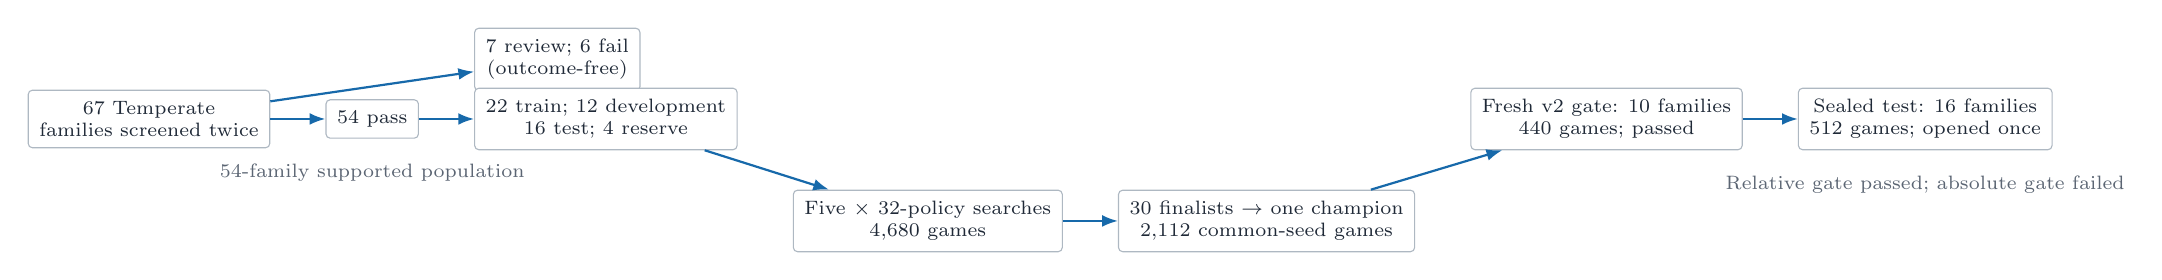
\begin{tikzpicture}[
  node distance=4mm and 7mm,
  box/.style={draw=ChronoGrid,rounded corners=1.5pt,fill=white,text=ChronoInk,align=center,font=\scriptsize,inner sep=4pt},
  arrow/.style={-{Latex[length=2mm]},draw=ChronoBlue,line width=0.8pt},
  note/.style={text=ChronoMuted,font=\scriptsize,align=center}
]
\node[box] (screen) {67 Temperate\\families screened twice};
\node[box,right=of screen] (pass) {54 pass};
\node[box,above right=1mm and 7mm of pass] (exclude) {7 review; 6 fail\\(outcome-free)};
\node[box,right=of pass] (roles) {22 train; 12 development\\16 test; 4 reserve};
\node[box,below right=5mm and 7mm of roles] (search) {Five $\times$ 32-policy searches\\4,680 games};
\node[box,right=of search] (championship) {30 finalists $\rightarrow$ one champion\\2,112 common-seed games};
\node[box,above right=5mm and 7mm of championship] (dev) {Fresh v2 gate: 10 families\\440 games; passed};
\node[box,right=of dev] (test) {Sealed test: 16 families\\512 games; opened once};
\draw[arrow] (screen) -- (pass);
\draw[arrow] (screen) -- (exclude);
\draw[arrow] (pass) -- (roles);
\draw[arrow] (roles) -- (search);
\draw[arrow] (search) -- (championship);
\draw[arrow] (championship) -- (dev);
\draw[arrow] (dev) -- (test);
\node[note,below=2mm of pass] {54-family supported population};
\node[note,below=2mm of test] {Relative gate passed; absolute gate failed};
\end{tikzpicture}
}
  \caption{Outcome-access and family flow. The 12-family initial development
  role was used by a retired method-v1 selector. Method v2 used the 22 training
  families and a fresh pool formed from four original reserves plus seven
  technically admissible review families; it opened the 16 test families only
  after the frozen development gate passed. Counts refer to the finalized
  accepted path.}
  \label{fig:flow}
\end{figure}

\subsection{Fail-closed provenance}

Each plan binds the Git source, compiled JavaScript, lockfile, Node executable,
game API, external opponent tree, map bytes, policy, family role, seeds, slot,
environment allowlist, and intended Slurm account. Every shard emits atomic
intent, launch, completion, summary, and terminal records. Reducers require the
exact planned set and query Slurm for authoritative account and job IDs. An
in-run retry is forbidden. A scheduler attempt may be repeated only if it is
proven to have stopped before its first counted launch; a post-launch technical
failure invalidates the indivisible campaign rather than permitting selective
repair. Superseded and failed attempts remain in the ledger.

\section{StrongBot and Experimental Method}
\label{sec:method}

\subsection{Layered policy}

StrongBot retains Supalosa's base-building, economy, scouting, defense, and
attack-mission machinery, then dispatches narrow policy layers from public map
and start state. The dispatch is deterministic and uses exact start-location
signatures rather than a learned map classifier.

\paragraph{West rush and home guard.}
On HFO west, the baseline often attacks before protecting its exposed base or
banks resources behind a slow macro plan. The selected Allied and Soviet
profiles use rush planning with HFO force composition and a grouped home guard.
The guard reserves a local force around fixed home anchors during the opening;
the remaining force can attack. Allied and Soviet permissions are separate so
one faction's profile cannot alter the other's behavior.

\paragraph{Progress-gated building retarget.}
HFO bottom produced long advantages that failed to close. After update 42,000,
the controller becomes eligible only when at most six enemy buildings and four
enemy combatants remain, at least four non-dog attackers are available, and
the attacking force is noninferior. It tracks both enemy building count and
aggregate building hit points. If neither improves for 1,200 updates, the
controller activates; after another 600-update stall it rotates to a
deterministically ranked building and reissues attack orders. Progress resets
the stall clock. This is a liveness repair with explicit safety conditions, not
an unconditional attack-everything rule.

\paragraph{Literal closeout.}
Late-game routines distinguish selectable combatants from buildings, retain
home defense when threats remain, and direct surplus combatants toward
remaining structures. The objective is not to destroy every enemy unit. If
the final building is eliminated first, the game is already won; if blocking
forces prevent access, they may need to be cleared before the building strike.

\paragraph{Peak reciprocal macro scope.}
The Peak macro profile was originally applied only at start \texttt{(37,73)}.
The confirmed policy applies the same immutable macro profile at both exact
Peak starts. Bot/tactical scope remains \texttt{weak\_only}. Thus the selected
change is one predicate: the reciprocal start receives an existing strategy,
not a newly tuned parameter set.

\begin{algorithm}[t]
\DontPrintSemicolon
\KwIn{public state $s$, update $u$, exact map/start, country}
$p \leftarrow$ frozen map--start--country profile\;
\If{Peak and either registered reciprocal start}{
  set only $p.\texttt{strategyScope}\leftarrow\texttt{both}$\;
}
run inherited economy, production, defense, and mission update under $p$\;
\If{HFO west}{
  use the faction-specific rush plan and reserve the grouped home guard\;
}
\If{HFO bottom, $u\geq42{,}000$, and force/building safety gates pass}{
  update building-count and building-hit-point progress clocks\;
  \If{no progress for 1,200 updates}{
    activate building retarget; rotate after each further 600-update stall\;
  }
}
\If{late game and opponent buildings remain}{
  retain required home defense and send surplus combatants to ranked structures\;
}
\caption{StrongBot's deterministic policy composition. Every branch is scoped
by immutable public map/start/faction state; no opponent identity or hidden
engine field enters dispatch.}
\label{alg:strongbot}
\end{algorithm}

\subsection{Prospective development gates}

Each mechanism follows the same sequence:

\begin{enumerate}
  \item freeze candidate arms, seed namespace, strata, endpoint, uncertainty,
  and advancement rule before new outcomes;
  \item select exact starts without updating the game or writing W/D/L;
  \item run every paired cell once and inspect only the complete aggregate;
  \item replicate the unchanged winner on fresh cases; and
  \item run an outcome-free activation-isolation gate, requiring a changed
  action trace in every intended-active country--start cell and exact
  action/state/production equality in every intended-inactive cell.
\end{enumerate}

Table~\ref{tab:mechanisms} reports the final replicated screens. The paired
lower column is the prespecified one-sided 95\% t lower bound on W/D/L score
difference. Inactive exact is the number of non-target country--start cells
with identical normalized traces.

\begin{table*}[t]
\centering
\caption{Replicated scoped mechanisms and outcome-free isolation. Controls and
winners use the same cases and random streams.}
\label{tab:mechanisms}
\small
\begin{tabular}{@{}lrrrr@{}}
\toprule
Mechanism & Control W/D/L & Winner W/D/L & Paired lower & Inactive exact \\
\midrule
Allied west rush+guard & 1/11/38 & 47/2/1 & +0.764 & 31 \\
Soviet west rush+guard & 47/43/30 & 98/9/13 & +0.211 & 32 \\
Bottom progress retarget & 123/98/49 & 198/23/49 & +0.115 & 27 \\
\bottomrule
\end{tabular}

\end{table*}

Allied west improves from \AlliedControlWdl{} to \AlliedWinnerWdl{}
(\AlliedPairedLower{} lower bound) and is exact in
\AlliedInactiveCells{} inactive cells. Soviet west improves from
\SovietControlWdl{} to \SovietWinnerWdl{} (\SovietPairedLower{}) with
\SovietInactiveCells{} inactive cells. Bottom retarget improves
\BottomControlWdl{} to \BottomWinnerWdl{} (\BottomPairedLower{}) while holding
losses at 49 and remaining exact in \BottomInactiveCells{} inactive cells.
These studies authorize deployment; they are not substitutes for the complete
HFO confirmation.

\subsection{Final evaluations and uncertainty}

The frozen HFO confirmation contains 720 fresh games: ten cases in each of
$9$ countries $\times 4$ candidate starts $\times 2$ participant slots.
We report pooled W/D/L, one-sided 95\% Wilson lower bounds for win rates, and an
equal-weight country-by-start mean with Student-t lower bound over 36 cells.
Country, start, side, and slot strata were prespecified.

For a matched policy comparison, let
$d_i=s_i^{(1)}-s_i^{(0)}$ for case score $s_i\in\{0,0.5,1\}$. The
one-sided 95\% paired lower bound is
$\bar d-t_{0.95,n-1}s_d/\sqrt{n}$. For an equal-weight country--start
bound, we first average literal win indicators within each cell, then apply the
analogous one-sided Student-$t$ bound to the 36 HFO or 18 Peak cell means,
against null 0.5. Pooled literal win rates use one-sided Wilson bounds. Thus
games are paired where policies share a case, while country--start cells are
the generalization units for the reported spatial lower bounds.

Peak Stage~0 tests six frozen arms on 36 development cases. Four arms form a
$2\times2$ factorial of macro scope and bot/tactical scope; two reproduce a
historical defensive-infantry candidate. Eligible arms must improve paired
score, reduce losses, be positive at both starts/sides/slots, be noninferior in
every country, and be trajectory-identical at the already-profiled start.
Exactly one arm is selected by a fixed ranking. Replication compares that
unchanged arm with deployed control on 180 fresh cases, five per
country--start--slot cell. Its final gate additionally requires pooled,
paired, and 18-cell country-by-start lower bounds above their nulls.

The Advanced experiment pairs StrongBot and pinned Supalosa against the same
frozen independent opponent on 360 fresh HFO cases each. It tests transfer; it
does not participate in candidate selection.

\section{Held-Out Results}
\label{sec:results}

All 128 confirmatory shards completed under the single prespecified Slurm
project account, with exactly 512 launches and completions, no failed task,
no additional attempt, and one irreversible unblinding. Table~\ref{tab:main}
reports both prespecified endpoints.

\begin{table}[t]
\centering
\caption{Frozen confirmatory result on 16 sealed families. W/D/L counts are
descriptive; inference treats the map family as the cluster.}
\label{tab:main}
\small
\begin{tabular}{@{}lrrrrl@{}}
\toprule
Quantity & Score/effect & W & D & L & Uncertainty / decision \\
\midrule
Default & \DefaultScore{} & \DefaultWins{} & \DefaultDraws{} & \DefaultLosses{} & descriptive \\
Champion & \ChampionScore{} & \ChampionWins{} & \ChampionDraws{} & \ChampionLosses{} & descriptive \\
Champion $-$ default & \ImprovementEstimate{} & & & &
95\% CI [\ImprovementCILower{}, \ImprovementCIUpper{}]; pass \\
Champion $-$ 0.5 & \ChampionAbsoluteMargin{} & & & &
one-sided 95\% lower \ChampionAbsoluteLower{}; fail \\
\bottomrule
\end{tabular}
\end{table}

\subsection{Relative improvement passes}

The default scores \DefaultScore{} (1 win, 100 draws, 155 losses), whereas the
champion scores \ChampionScore{} (47 wins, 180 draws, 29 losses). The
equally-family-weighted champion-minus-default estimate is
\ImprovementEstimate{}, with clustered standard error \ImprovementSE{} and
95\% interval [\ImprovementCILower{},~\ImprovementCIUpper{}]. Its lower endpoint
is above zero, passing the relative gate.

Figure~\ref{fig:family-effects} shows every family effect. Fourteen are
positive, two are exactly zero, and none is negative at the family-average
level. Effects range from 0 to 0.844; thus the mean is not produced by a single
family, although effect magnitude is heterogeneous. These points are estimates
from 16 games per method and family, not independent confidence intervals.

\begin{figure}[t]
  \centering
  
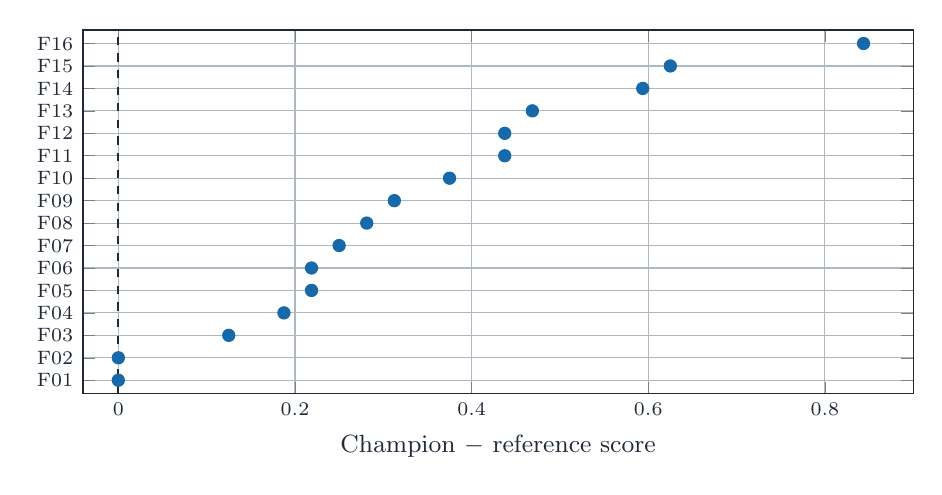
\begin{tikzpicture}
\begin{axis}[
  width=\linewidth,
  height=6.2cm,
  xmin=-0.04, xmax=0.90,
  ymin=0.4, ymax=16.6,
  xtick={0,0.2,0.4,0.6,0.8},
  ytick={1,2,3,4,5,6,7,8,9,10,11,12,13,14,15,16},
  yticklabels={F01,F02,F03,F04,F05,F06,F07,F08,F09,F10,F11,F12,F13,F14,F15,F16},
  xlabel={Champion $-$ reference score},
  axis line style={draw=ChronoInk},
  tick label style={text=ChronoInk,font=\scriptsize},
  label style={text=ChronoInk,font=\small},
  grid=major,
  grid style={draw=ChronoGrid},
  clip=false
]
\addplot[draw=ChronoInk,dashed,line width=0.7pt] coordinates {(0,0.4) (0,16.6)};
\addplot[only marks,mark=*,mark size=2.2pt,draw=ChronoBlue,fill=ChronoBlue]
  coordinates {(0.00000000,1) (0.00000000,2) (0.12500000,3) (0.18750000,4) (0.21875000,5) (0.21875000,6) (0.25000000,7) (0.28125000,8) (0.31250000,9) (0.37500000,10) (0.43750000,11) (0.43750000,12) (0.46875000,13) (0.59375000,14) (0.62500000,15) (0.84375000,16)};
\end{axis}
\end{tikzpicture}

  \caption{Champion-minus-default score on each sealed family, ordered by
  effect. Labels map to public family IDs in the supplement. The dashed line is
  zero; no game-level error bars are shown because the prespecified inference
  clusters at the family level.}
  \label{fig:family-effects}
\end{figure}

As post-confirmatory sensitivity checks, an independent Python reducer reread
all 512 raw completion records and reproduced the point estimates, standard
errors, and bounds exactly. A 100,000-replicate family bootstrap yielded a 95\%
interval [\ImprovementBootstrapLower{},~\ImprovementBootstrapUpper{}], and the
exact family sign-flip two-sided value was
$p=\ImprovementSignFlipP{}$. These checks support robustness of the relative
result but did not replace the frozen estimator.

\subsection{Absolute superiority does not pass}

The champion's score margin over 0.5 is \ChampionAbsoluteMargin{}, with
family-clustered standard error 0.032. Its prespecified one-sided 95\% lower
bound is \ChampionAbsoluteLower{}, so the absolute-strength gate fails. Six
family scores are above 0.5, five equal 0.5, and five fall below 0.5. The
diagnostic family-bootstrap interval for champion score, [0.482, 0.604], leads
to the same caution. Therefore, the correct result is not ``StrongBot reliably
beats Supalosa.'' It is ``the configured StrongBot robustly improves its
shipped default against pinned Supalosa on this family population.''

\subsection{The gain is mostly avoided losses}

Because both methods use the same family, engine seed, opponent stream, and
physical slot, the 256 per-method games form direct outcome pairs.
Figure~\ref{fig:transitions} shows their transition matrix. Of 155 default
losses, 104 become champion draws and 28 become champion wins. Eighteen default
draws become wins, while six regress to losses. Overall, \ImprovedPairCount{}
pairs improve, \RegressedPairCount{} regress, and \UnchangedPairCount{} have
the same frozen score. The policy gains 46 wins and avoids 126 losses relative
to default, but its most common improvement is loss-to-tick-cap survival.

\begin{figure}[t]
  \centering
  
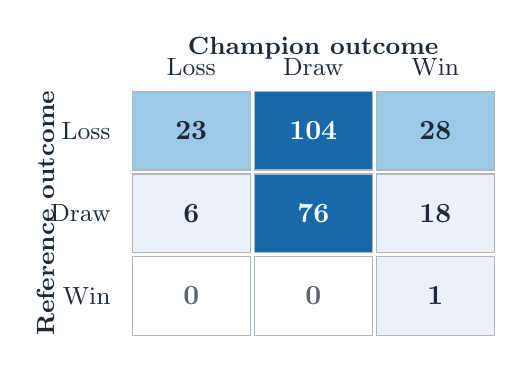
\begin{tikzpicture}[font=\sffamily]
\node[anchor=east,text=ChronoInk,font=\small] at (-0.9,0.0) {Loss};
\node[anchor=east,text=ChronoInk,font=\small] at (-0.9,-1.05) {Draw};
\node[anchor=east,text=ChronoInk,font=\small] at (-0.9,-2.1) {Win};
\node[anchor=south,text=ChronoInk,font=\small] at (0.0,0.57) {Loss};
\node[anchor=south,text=ChronoInk,font=\small] at (1.55,0.57) {Draw};
\node[anchor=south,text=ChronoInk,font=\small] at (3.1,0.57) {Win};
\node[draw=ChronoGrid,fill=ChronoBlueLight,text=ChronoInk,minimum width=1.5cm,minimum height=1cm,font=\bfseries] at (0.0,0.0) {23}; \node[draw=ChronoGrid,fill=ChronoBlue,text=white,minimum width=1.5cm,minimum height=1cm,font=\bfseries] at (1.55,0.0) {104}; \node[draw=ChronoGrid,fill=ChronoBlueLight,text=ChronoInk,minimum width=1.5cm,minimum height=1cm,font=\bfseries] at (3.1,0.0) {28}; \node[draw=ChronoGrid,fill=ChronoPale,text=ChronoInk,minimum width=1.5cm,minimum height=1cm,font=\bfseries] at (0.0,-1.05) {6}; \node[draw=ChronoGrid,fill=ChronoBlue,text=white,minimum width=1.5cm,minimum height=1cm,font=\bfseries] at (1.55,-1.05) {76}; \node[draw=ChronoGrid,fill=ChronoPale,text=ChronoInk,minimum width=1.5cm,minimum height=1cm,font=\bfseries] at (3.1,-1.05) {18}; \node[draw=ChronoGrid,fill=white,text=ChronoMuted,minimum width=1.5cm,minimum height=1cm,font=\bfseries] at (0.0,-2.1) {0}; \node[draw=ChronoGrid,fill=white,text=ChronoMuted,minimum width=1.5cm,minimum height=1cm,font=\bfseries] at (1.55,-2.1) {0}; \node[draw=ChronoGrid,fill=ChronoPale,text=ChronoInk,minimum width=1.5cm,minimum height=1cm,font=\bfseries] at (3.1,-2.1) {1};
\node[rotate=90,text=ChronoInk,font=\small\bfseries] at (-1.85,-1.05) {Reference outcome};
\node[text=ChronoInk,font=\small\bfseries] at (1.55,1.05) {Champion outcome};
\end{tikzpicture}

  \caption{Paired outcome transitions over 256 matched
  family--seed--slot cells. Rows are default outcomes; columns are champion
  outcomes. Cell shading reflects count and all counts, including zeros, are
  shown.}
  \label{fig:transitions}
\end{figure}

\section{Post-Confirmatory Diagnostics}
\label{sec:diagnostics}

The analyses in this section were specified or conducted after the held-out
result. They explain and stress-test the frozen policy; they do not alter its
selection or rescue the failed absolute gate.

\subsection{Does the common-seed championship help?}

The championship addressed a training-only concern: each optimizer run had
selected its six finalists under different seeds. We therefore compared the
champion with the five policies that each run would have selected on its own,
using four new common seed blocks on the ten open method-v2 development
families. The complete design contains \MechanismGameCount{} games (six
methods, ten families, four seed blocks, and reciprocal slots).

The champion scores \MechanismChampionScore{}, compared with
\MechanismLocalAverageScore{} for the equal average of the
five run-local policies. The difference is \MechanismEstimate{}, but its
family-clustered 95\% interval
[\MechanismCILower{},~\MechanismCIUpper{}] includes zero. All five pairwise
point differences favor the champion (\MechanismPairwiseMinimum{} to
\MechanismPairwiseMaximum{}), while every pairwise
interval crosses zero. This evidence is consistent with common-seed selection
being useful, but ten families do not statistically resolve the mechanism.

\subsection{Which policy group matters?}

We formed five policies that each revert one group of champion settings to the
default: defense-radius growth, emergency defense, forced attack, scouting, or
the joint attack-composition/strategic-plan group. A second 480-game
common-seed panel compared all reverts with the champion on the same ten open
families. The primary champion-minus-equal-revert-average estimate is
\ComponentAverageEstimate{} with 95\% interval
[\ComponentAverageCILower{},~\ComponentAverageCIUpper{}].

Figure~\ref{fig:components} reports every individual contrast. Reverting
infantry+rush to assault/macro gives by far the largest decline:
\StrategyEstimate{}, with ordinary 95\% interval
[\StrategyOrdinaryLower{},~\StrategyOrdinaryUpper{}]. However, its
prespecified five-comparison Bonferroni familywise interval is
[\StrategyFamilywiseLower{},~\StrategyFamilywiseUpper{}], narrowly including
zero. The defense-growth and forced-attack reverts have slightly higher point
scores than the champion, emergency defense is near zero, and the scouting
revert is endpoint-identical in all 80 paired games. Thus the joint strategy
group is the dominant observed signal, but no individual component clears the
multiplicity-controlled criterion.

\begin{figure}[t]
  \centering
  
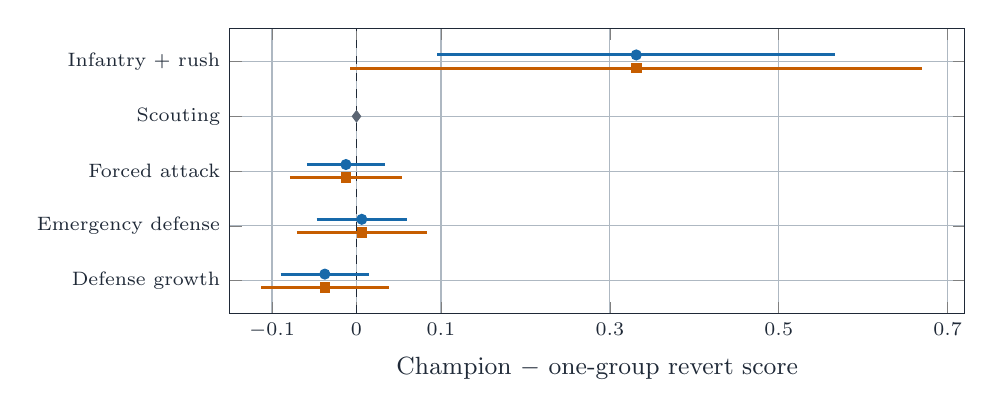
\begin{tikzpicture}
\begin{axis}[
  width=0.90\linewidth,
  height=5.2cm,
  xmin=-0.15, xmax=0.72,
  ymin=0.4, ymax=5.6,
  xtick={-0.1,0,0.1,0.3,0.5,0.7},
  ytick={1,2,3,4,5},
  yticklabels={{Defense growth},{Emergency defense},{Forced attack},{Scouting},{Infantry + rush}},
  xlabel={Champion $-$ one-group revert score},
  axis line style={draw=ChronoInk},
  tick label style={text=ChronoInk,font=\scriptsize},
  label style={text=ChronoInk,font=\small},
  grid=major,
  grid style={draw=ChronoGrid},
  clip=false
]
\addplot[draw=ChronoInk,dashed,line width=0.7pt] coordinates {(0,0.4) (0,5.6)};
\draw[ChronoBlue,line width=1.1pt] (axis cs:-0.08997983,1.12) -- (axis cs:0.01497983,1.12); \addplot[only marks,mark=*,mark size=1.8pt,draw=ChronoBlue,fill=ChronoBlue] coordinates {(-0.03750000,1.12)}; \draw[ChronoOrange,line width=1.1pt] (axis cs:-0.11289299,0.88) -- (axis cs:0.03789299,0.88); \addplot[only marks,mark=square*,mark size=1.7pt,draw=ChronoOrange,fill=ChronoOrange] coordinates {(-0.03750000,0.88)}; \draw[ChronoBlue,line width=1.1pt] (axis cs:-0.04727743,2.12) -- (axis cs:0.05977743,2.12); \addplot[only marks,mark=*,mark size=1.8pt,draw=ChronoBlue,fill=ChronoBlue] coordinates {(0.00625000,2.12)}; \draw[ChronoOrange,line width=1.1pt] (axis cs:-0.07064799,1.88) -- (axis cs:0.08314799,1.88); \addplot[only marks,mark=square*,mark size=1.7pt,draw=ChronoOrange,fill=ChronoOrange] coordinates {(0.00625000,1.88)}; \draw[ChronoBlue,line width=1.1pt] (axis cs:-0.05867609,3.12) -- (axis cs:0.03367609,3.12); \addplot[only marks,mark=*,mark size=1.8pt,draw=ChronoBlue,fill=ChronoBlue] coordinates {(-0.01250000,3.12)}; \draw[ChronoOrange,line width=1.1pt] (axis cs:-0.07883699,2.88) -- (axis cs:0.05383699,2.88); \addplot[only marks,mark=square*,mark size=1.7pt,draw=ChronoOrange,fill=ChronoOrange] coordinates {(-0.01250000,2.88)}; \addplot[only marks,mark=diamond*,mark size=2pt,draw=ChronoMuted,fill=ChronoMuted] coordinates {(0.00000000,4)}; \draw[ChronoBlue,line width=1.1pt] (axis cs:0.09556151,5.12) -- (axis cs:0.56693849,5.12); \addplot[only marks,mark=*,mark size=1.8pt,draw=ChronoBlue,fill=ChronoBlue] coordinates {(0.33125000,5.12)}; \draw[ChronoOrange,line width=1.1pt] (axis cs:-0.00734223,4.88) -- (axis cs:0.66984223,4.88); \addplot[only marks,mark=square*,mark size=1.7pt,draw=ChronoOrange,fill=ChronoOrange] coordinates {(0.33125000,4.88)};
\end{axis}
\end{tikzpicture}

  \caption{Champion-minus-one-group-revert effects. Blue circles/lines are
  ordinary family-clustered 95\% intervals; orange squares/lines are
  Bonferroni familywise-95\% intervals. The scouting contrast (gray diamond)
  has zero endpoint difference and zero observed variance, so no artificial
  interval is drawn.}
  \label{fig:components}
\end{figure}

\subsection{Terminal army and economy pattern}

A deterministic analyzer validated and reduced all \TerminalRawRecordCount{} raw completion
records from the confirmatory and two diagnostic panels. Across confirmatory
pairs, the champion improves its candidate-minus-opponent terminal balance by
\ConfirmatoryTerminalCombatantDifference{} combatants and
\ConfirmatoryTerminalUnitDifference{} total units while holding
\ConfirmatoryTerminalCreditReduction{} fewer credits.
Outcome changes mechanically alter terminal snapshots, so we also examine the
\StableDrawPairCount{} pairs that remain tick-cap draws under both methods.
They have identical score and duration, yet the champion ends with
\StableDrawCombatantDifference{} more relative combatants,
\StableDrawUnitDifference{} more relative units, and
\StableDrawCreditDifference{} relative credits.

The strategy-revert panel has the same qualitative pattern: the champion has
\StrategyTerminalCombatantDifference{} more relative combatants,
\StrategyTerminalUnitDifference{} more relative units, and
\StrategyTerminalCreditReduction{} fewer credits overall. These endpoints
are consistent with converting banked
resources into fielded combat power. They do not establish when or how that
conversion occurred, because the preserved games contain no action trace,
production timeline, combat log, or intermediate state trajectory. Likewise,
endpoint identity for the scouting revert does not prove identical internal
actions.

\section{Reproducibility, Limitations, and Release}
\label{sec:limitations}

\subsection{Execution and artifact chain}

The finalized accepted path contains \TotalGameCount{} policy games:
\OptimizerGameCount{} in the five searches, \ChampionshipGameCount{} in the
championship, \DevelopmentGameCount{} in fresh development,
\ConfirmatoryGameCount{} in confirmatory evaluation, and
\MechanismGameCount{} in each diagnostic panel. All accepted shards
ran under the single prespecified Slurm project account; plan, event, summary,
scheduler,
and raw-completion counts agree, and no accepted campaign contains a technical
failure or extra attempt. Two zero-launch campaigns and one sealed development
campaign with a deterministic post-launch map-extension interface failure are
retained separately. The latter was retired as an indivisible campaign; after
a prospective interface repair, the full development protocol restarted from
phase 1 without inspecting or pooling its outcomes.

Every interpreted result maps to an exact configuration, source revision,
opponent revision, artifact hash, and Slurm job ID in an append-only registry.
Paper macros and TikZ/PGFPlots fragments are generated from committed JSON
artifacts. The generator pins input hashes, cross-checks overlapping
aggregates, and emits an output manifest; tests fail on numerical drift. A
clean artifact can therefore reproduce every table and figure without the
private cluster paths or raw third-party assets.

The intended release includes author-owned bot changes, orchestration,
protocols, tests, manifests, hashes, family metadata, aggregate results, and
paper-generation code. Chrono Divide code, Supalosa code, Red Alert 2 archives,
and downloaded map files remain under their respective rights. We will provide
acquisition and hash-verification instructions rather than redistributing
third-party content without permission. For double-blind review, the artifact
will use an identity-neutral archive and contain no author-identifying URL or
metadata.

\subsection{Limitations}

\paragraph{One opponent and matchup.}
Supalosa is the only independent bot and all games are Iraq mirrors. The test
therefore estimates one pinned opponent/faction matchup, not general agent
strength; the failed absolute gate emphasizes this boundary.

\paragraph{Supported map population.}
Only Temperate families passing two compatibility screens are included; Snow,
Urban, and Desert lack complete authorized asset/runtime support. Family
grouping is a conservative heuristic, and tick-250 compatibility is not proof
of full behavioral fidelity to commercial Red Alert 2.

\paragraph{Comparator boundary.}
The reference is candidate 0 inside the coordinate-free research interface,
not the fork's map-profile-enabled deployed default. This comparison isolates
configuration within the declared generic policy class, but it does not
estimate improvement over the deployed policy; the reference's low score can
make the relative gain appear larger than a product-level improvement.

\paragraph{High draw rate and endpoint.}
The 18,000-tick cap produces many draws, all scored 0.5 regardless of terminal
advantage. The primary gain is often survival rather than elimination. A
different cap or outcome definition could answer a different question; neither
was varied after results.

\paragraph{Algorithmic comparison.}
Successive halving, common random numbers, and deterministic selection are
known. Without a SMAC, irace, NTBEA, or hand-tuning comparator, we claim
neither search efficiency nor optimizer novelty. The tie term affects training
rankings only; held-out evaluation uses game score.

\paragraph{Adaptation and diagnostic power.}
Method v2 followed a negative development result for method v1. Test data
remained sealed and the new development pool was disjoint, but the final method
should be understood as a transparently adapted research program rather than a
single-shot preregistration. Component and championship diagnostics use only
ten open families, with intervals spanning zero; terminal snapshots lack
trajectories.

More seeds on opened tests would be post-selection without new generalization
units; future work needs prospectively screened maps, independent bots,
cross-faction matchups, and logged trajectories.

\section{Conclusion}

StrongBot reliably beats pinned Supalosa under literal all-building elimination
on two Chrono Divide maps. On HFO it wins \HfoWins{} of \HfoGames{} balanced
games, with pooled and country-by-start lower bounds above 0.84. On Peak, one
reciprocal macro-scope repair raises the win rate from \PeakControlWinRate{} to
\PeakWinRate{} on fresh paired cases, with a paired-score lower gain of
\PeakPairedLower{}. Replicated west rush/guard and bottom progress-retarget
studies, together with exact inactive-cell traces, connect these outcomes to
specific scoped mechanisms.

The result is deliberately not a claim of universal dominance. The same
StrongBot loses badly to RA2Web Advanced, and a preserved HFO replay still
fails to rebuild a finishing force before the tick cap. Chrono Divide is
therefore useful not because it makes agent improvement easy, but because it
supports full-game objectives, deterministic paired intervention, and
auditable failure analysis. The main lesson is practical: map-profiled RTS
strength can be made reliable when each intervention has a declared scope,
fresh replication, literal victory semantics, and a fail-closed evidence chain.
Opponent robustness and map coverage remain the next research problems.


\bibliographystyle{splncs04}
\bibliography{references}
\end{document}
